% L22eqv.tex
%
% Predrag created file				jul  9 2006
% $Author$ $Date$


\section{Small $L=22$ system {\rpo s}}
\label{s:L22}

\KS\ system $L = 22$ periodic on the full space is small but empirically 
large enough to exhibit persistent chaos.  $L=22$ is a sensible choice 
because In units of mean wavelength the size of this small system is about 
$ \tildeL/\sqrt{2}= 2.4758$ 2.5 wavelengths, so the dynamics is 
competition between wavenumbers 2 and 3. Because of the strong $k^4$ 
contraction in \KS\ we expect a small eigenvalues to be significant, rest 
are in the numerical noise. See figure~6 in \refref{Christiansen:97}.

% Davidchack and Crofts 
 We investigate this system in 16 to 64 complex Fourier modes (32 to 
128-dimensional system of real ODEs) truncation, and recheck the results 
by redoing the calculation with the double number of Fourier modes. % 
observe how many digits change. The \eqv\ points are accurate to at least 
to $10^{-11}$. Since Lapack is also double precision accurate, the 
accuracy of the first few eigenvalues is similar, and certainly in excess 
of 6 significant digits. % All digits stated in tables are significant.
The accuracy that can be reached is of order of 
$|a(\period{p},d_p) - a_0| 
 \approx \epsilon \exp(\Lyap_p \period{p})$, 
 where $\epsilon \approx 10^{-17}$ for double precision, $\lambda_p$ is 
the largest Lyapunov exponent, and $\period{p}$ the period.  With a good 
starting guess, Newton's method typically reaches that accuracy after 2-3 
iterates.

\subsection{\Eqva}

Numerically we find \eqv\ of wavenumber $k$ by (when it exists)
by using $sin( k x /\tildeL)$ as the initial guess for the Newton routine.

For $L = 22$ we find
3 unstable \eqva\ and a symmetric pair of unstable \reqva.
The \eqva\ {\nameit}2 and {\nameit}3 found here
essentially lie in the 2nd and 3rd Fourier component complex planes,
respectively, with very
small deformations from higher harmonics.
\RLD{recheck their $a_1$ content}

{\nameit}0 \eqv\  $u=0$ eigenvalues are all real:

$
\Lyap_k = (k/\tildeL)^2- (k/\tildeL)^4
\\
\Lyap_1 = .07491380653628918486
\\
\Lyap_2 = .21981716232383106179
\\
\Lyap_3 = .19519587589864859776
\\
\Lyap_4 = -.39814037184588659558
\\
\Lyap_5 = -2.11905802765905426195
\\
\cdots
\,.
$

There no wavenumber 1 \eqv\ {\nameit}1 (but there is a pair
of {\nameit}1 \reqva).

Wavenumber 2 \eqv\ {\nameit}2, with exponents 
\\
$\Lyap_i \pm \theta_i
=(
\\
  0.13903973 \pm i 0.23842023,
\\
  0,
\\
 -0.08402656 \pm i 0.16019413,
\\
 -0.11941393, 
\\
 -0.27112264 \pm i 0.35630716,
\\
 -2.01303043,
\\
 -2.03775342,
\\
 -5.63649418,
\cdots
)$
% Ruslan L Davidchack, 	10 Jul 2006 
% 2-wave steady state:
% 
% $(\Lyap_i \pm \theta_i)=
% (
%   0.13903972165535 \pm 0.23842023092014i, \\
%   0.00000000345431                    , \\
%  -0.08402654994820 \pm 0.16019413653788i, \\
%  -0.11941394469356                    , \\
%  -0.27112264064485 \pm 0.35630715566102i
% )$
%
\PC{not sure this comment makes sense, but anyway:
eigs either appear as complex pairs, or
real pairs, because of complex Fourier coefficients? Should we list
real pairs? Probably best to list them only once.}

{\nameit}2 \eqv\ is selfdual under $u(x) \to -u(-x)$ symmetry.

% Ruslan L Davidchack, 	10 Jul 2006 
See figure figs/steady\_states2.jpg

% Ruslan L Davidchack, 	10 Jul 2006 
Wavenumber 3 \eqv\ {\nameit}3, with exponents 
\\
$\Lyap_i \pm \theta_i=
(
  0.093346                    , \\
  0.093344                    , \\
  0.0                    , \\
 -0.412774                    , \\
 -0.610752 \pm 0.375874 i
\\
)$
{\nameit}3 maps into itself under $d/L = 1/3$
shift, {\nameit}2 under $d/L = 1/2$.


The unstable manifold plane
is traced out in \reffig{f:neighborhood2w}(a).
Computed the 2 expanding eigenvectors of the
\eqv\ {\nameit}2, as well as the 3rd, least contracting direction; then
translated and rotated Fourier modes into this coordinate frame,
plotted the unstbale manifold.
% trajectory there, both in the lab and the mean velocity frame.


 It is the unstable manifold of the \nameit 2
{\eqv}, drawn by tracing out a set of points along one of the complex
eigenvectors, that start close to it. Surprisingly, everybody goes connects
to the \nameit 2 shifts by 1/2 wavelength (d = L/4 = 5.5) but as we are in
infty dimensions they do it not as the usual homoclinic connection, but in
many (all?) possible intermediate ways. This might be a clue for how to
partition symbolic dynamics. Note also that in your L22-long.eps one seems
to come quite close to \nameit 2 {\eqv}, so it might be a very dominant
influence on the strange attractor dynamics


The appears to be a heteroclinic connection from \nameit 2 
{\eqv}
unstable spiral out straight into \nameit 3 {\eqv}
$\period{} = 76.6$ \rpo\ seems like a closeby
relative of this.
That also means that the relative shift between the two {\eqva} is
fixed, as far as this conection is concerned.

What is great about
this is that the \nameit 2 unstable manifold has a heteroclinic connection to itself 
$L/2$ shifted, but
even better, to \nameit 2, and \nameit 3 unstable manifold has a heteroclinic
connection to \nameit 2. 
It's really pretty. That makes for a rigid backbone - 
we hope this will help us develop a symbolic dynamics for rpo's.

It is very unlikely 
that a single 1-$d$ Poincar\'e section,
can do the job, 
previous work\rf{Lan:Thesis,LanCvi06}
always needed several sections.

The idea is that the local unstable plane gives 2 coordinates, the
least contracting direction (or one of a complex pair) gives the 3rd.

We need to construct the backbone of heteroclinic connections
first. They are not like 3-$d$ R\"ossler and Lorenz examples:
here one spirals out,
then spirals in - hopefully there will be intelligent Poincare sections
transverse to initial \nameit 2 (or \nameit 3) unstable manifold, mapping onto
Poincare sections of trajectories leaving again
the next \nameit 3 or \nameit 2 unstable manifold.


Check next what these 2 unstable eigenvectors for \nameit 3 eqv. are - when they
are equal in magnitude you expect a `star', all directions in their plane
going straight out. Do they all fall int \nameit 2 eqv?

% Ruslan:  10 Jul 2006
% 
% 119 KB     "long_orbit.jpg"
%  88 KB     "steady_states1.jpg"
%  84 KB     "steady_states2.jpg"
% 197 KB     "rpos1.jpg"
% ----------------------------------------

For all spatial plots color axis $u \in [-3, 3]$ is the same,
same time units and spatial width $L$.
For the steady states the magnitude of the \nameit 2 is quite 
a bit smaller than that of the \nameit 3.

On the 
	$[a_?,a_?]$ plane
	the $\sigma x = -x$ symmetry of \KSe\ is explicit.


steady\_states1.jpg shows the numerical evolution and, since the
traveling wave is very unstable, it disappears after awhile. 
The numerically exact solution is plotted in steady\_states2.jpg

rpos1.jpg is attached as a sample. 

As it looks, will not help us with partitioning, it seems, unless there is
a trajectory that hits the contracting direction - maybe
( -0.11941393,0)
head on.

Might want to look at this blowup in
the \nameit 2 slowest contraction
$   ( -0.08402656 \pm i 0.16019413)$
complex eigenvectors plane, check whether the
spiralling rotation agrees with the real/imaginary parts of eigenvalues.

Question is still - why does all of the unstable manifold of 
\nameit 2 eqv go back
into 
\nameit 2 eqv?

%%%%%%%%%%%%%%%%%%%%%%%%%%%%%%%%%%%%%%%%%%%%%%%%%%%%%%%%%%%%%%%%
\begin{figure}[h]
\centering
(a) 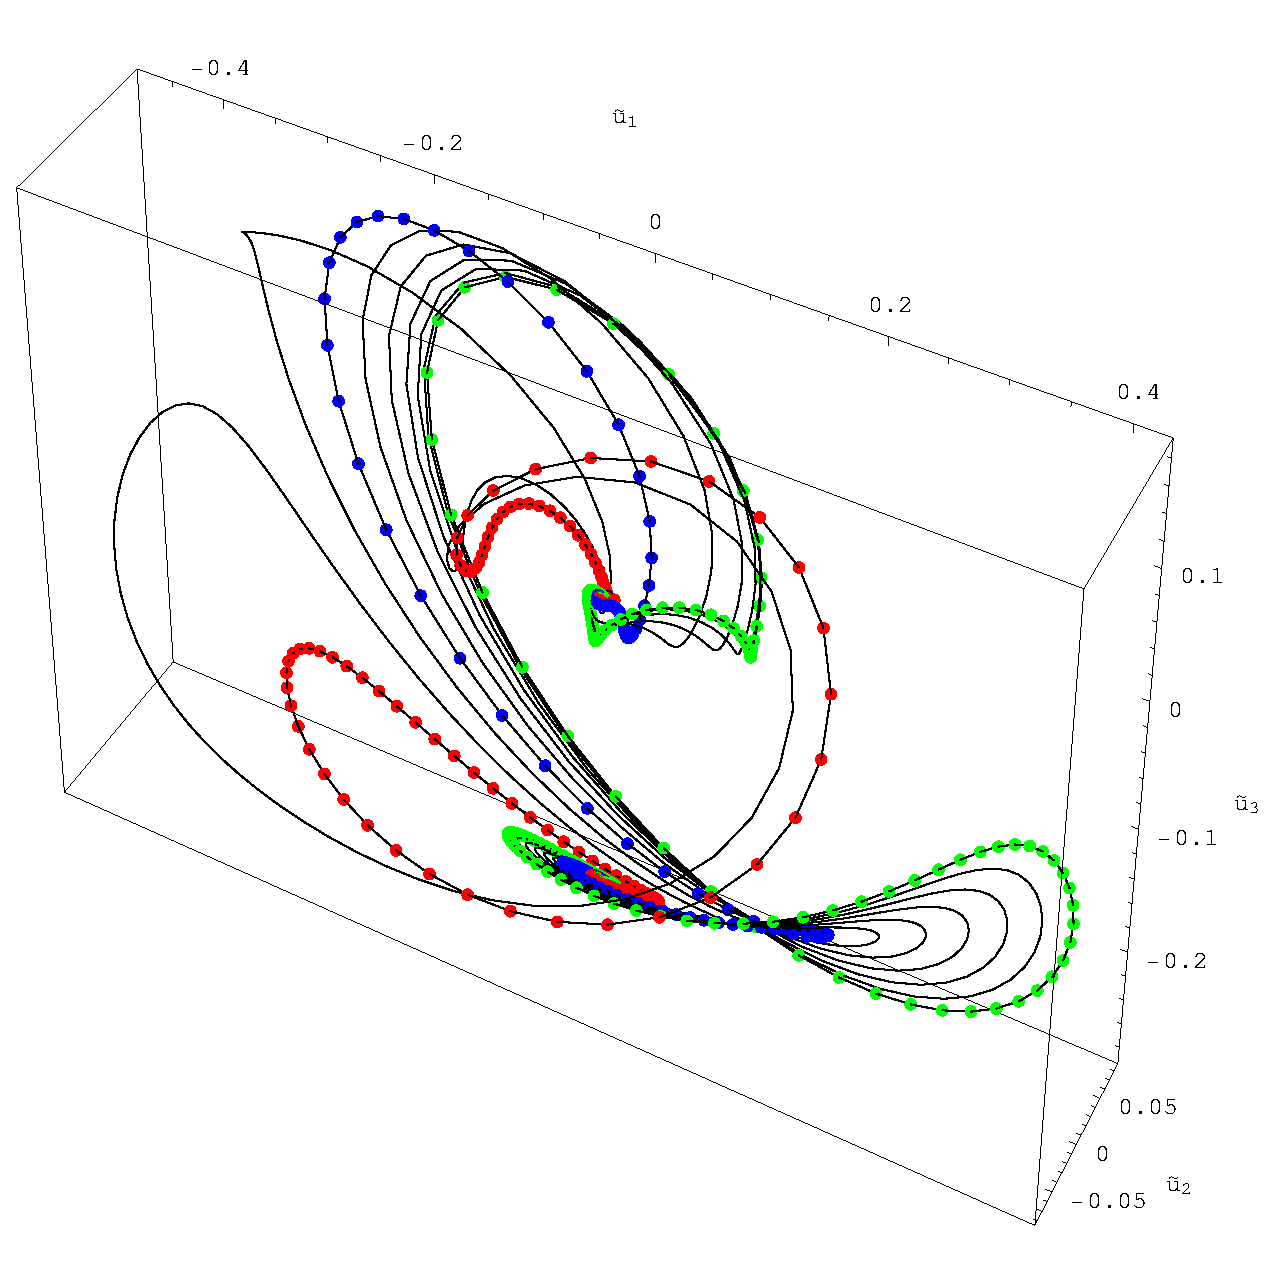
\includegraphics[width=5.0cm]{figs/L22-2w-UnsMan.eps}
\hspace{0.1in}
(b) 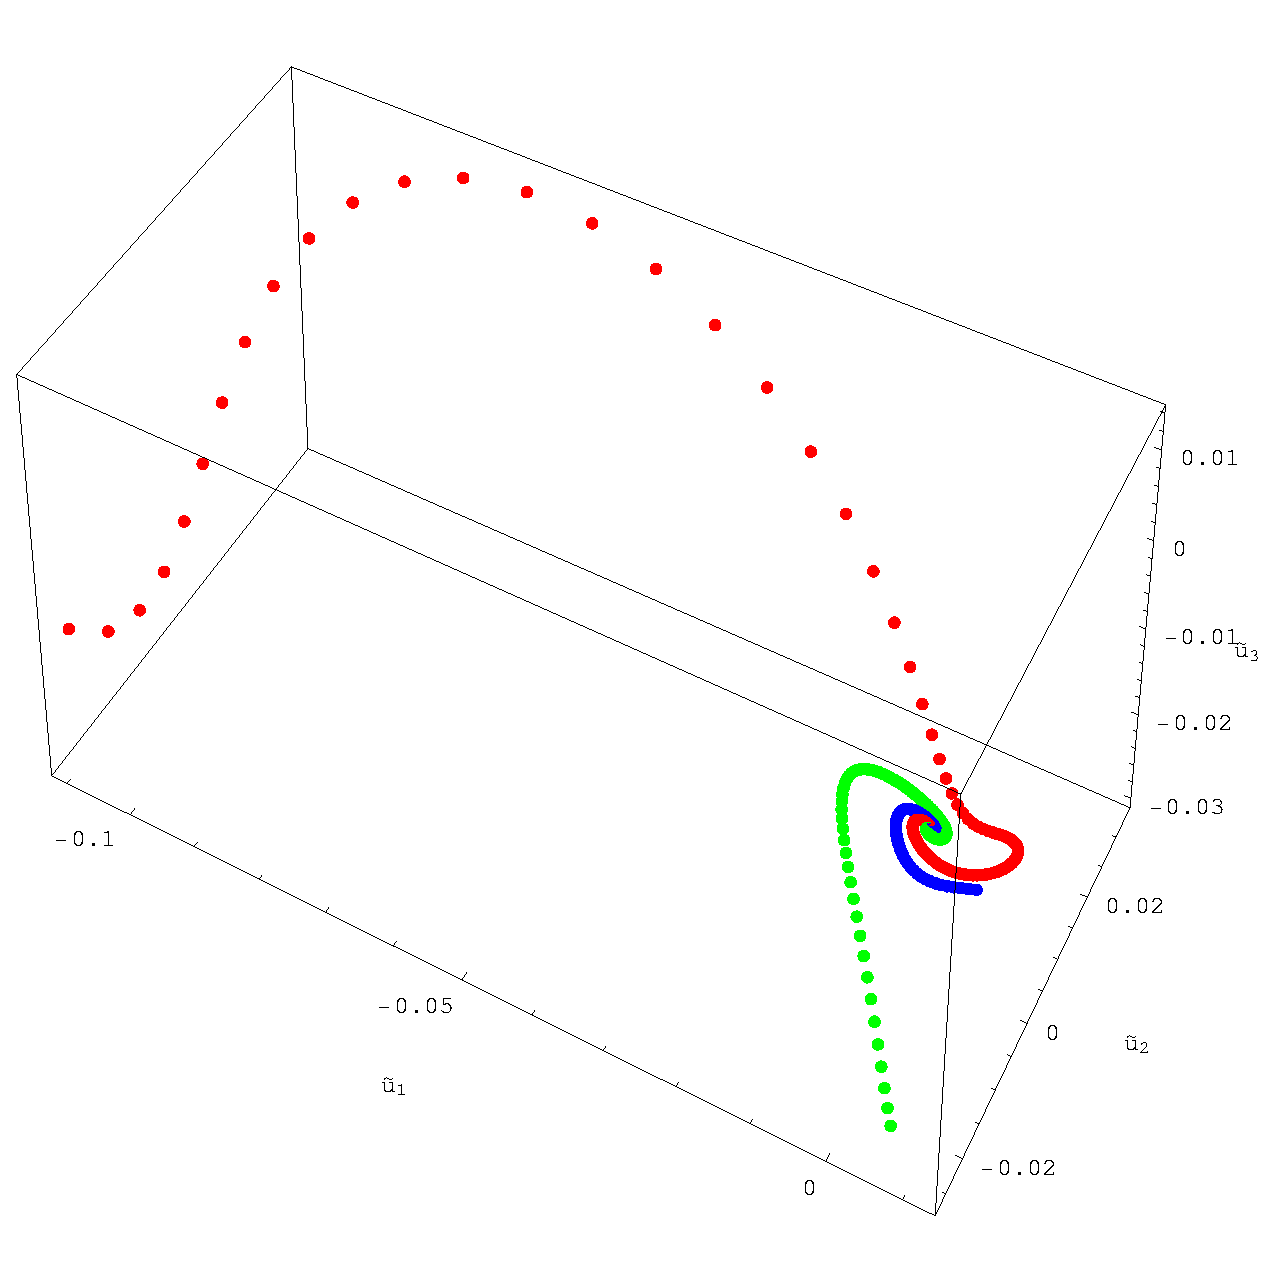
\includegraphics[width=5.0cm]{figs/L22-2w-UnsMan-BlowUp.eps}
% (b) 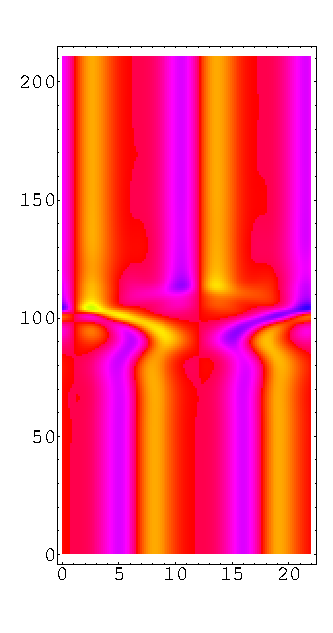
\includegraphics[width=4.0cm]{figs/L22-2w-R.eps}
\\
(c) 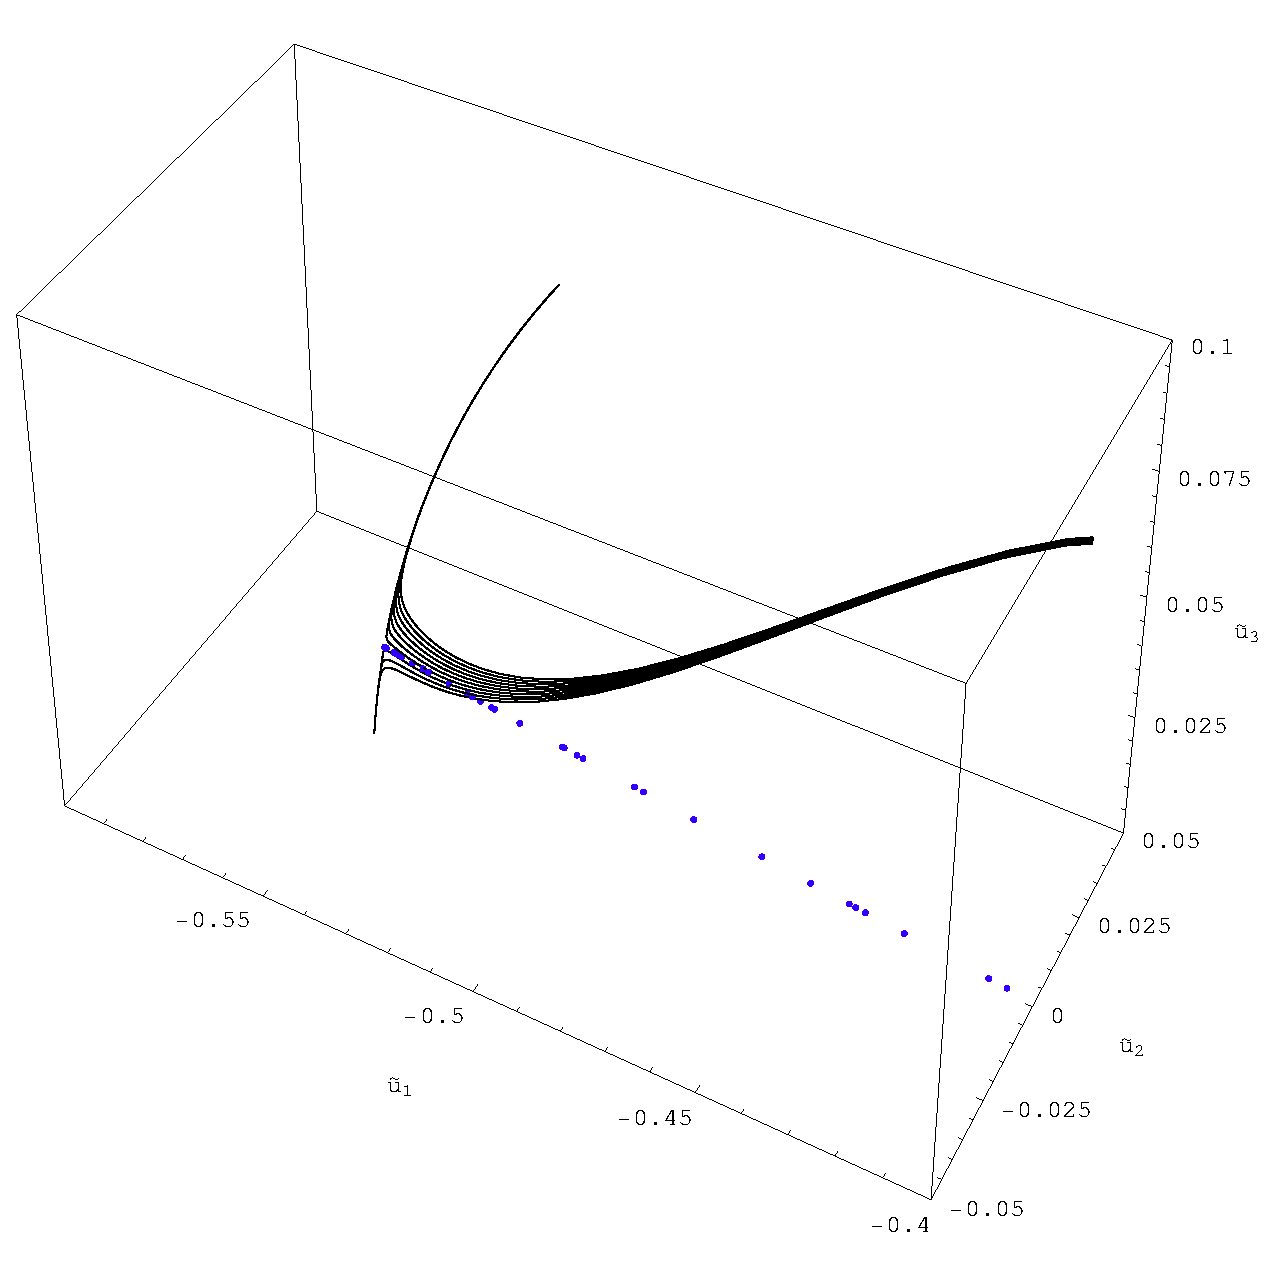
\includegraphics[width=5.0cm]{figs/L22-2w-3w-UnsMan.eps}
% (c) 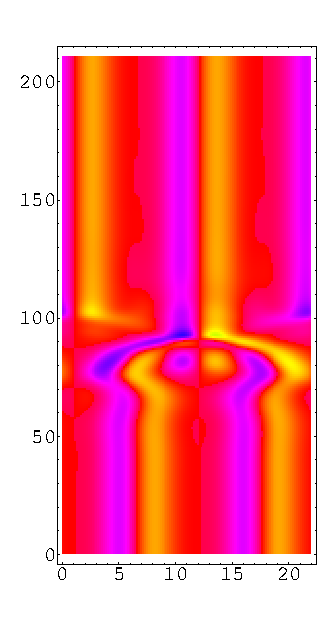
\includegraphics[width=4.0cm]{figs/L22-2w-G.eps}
\hspace{0.1in}
(d)  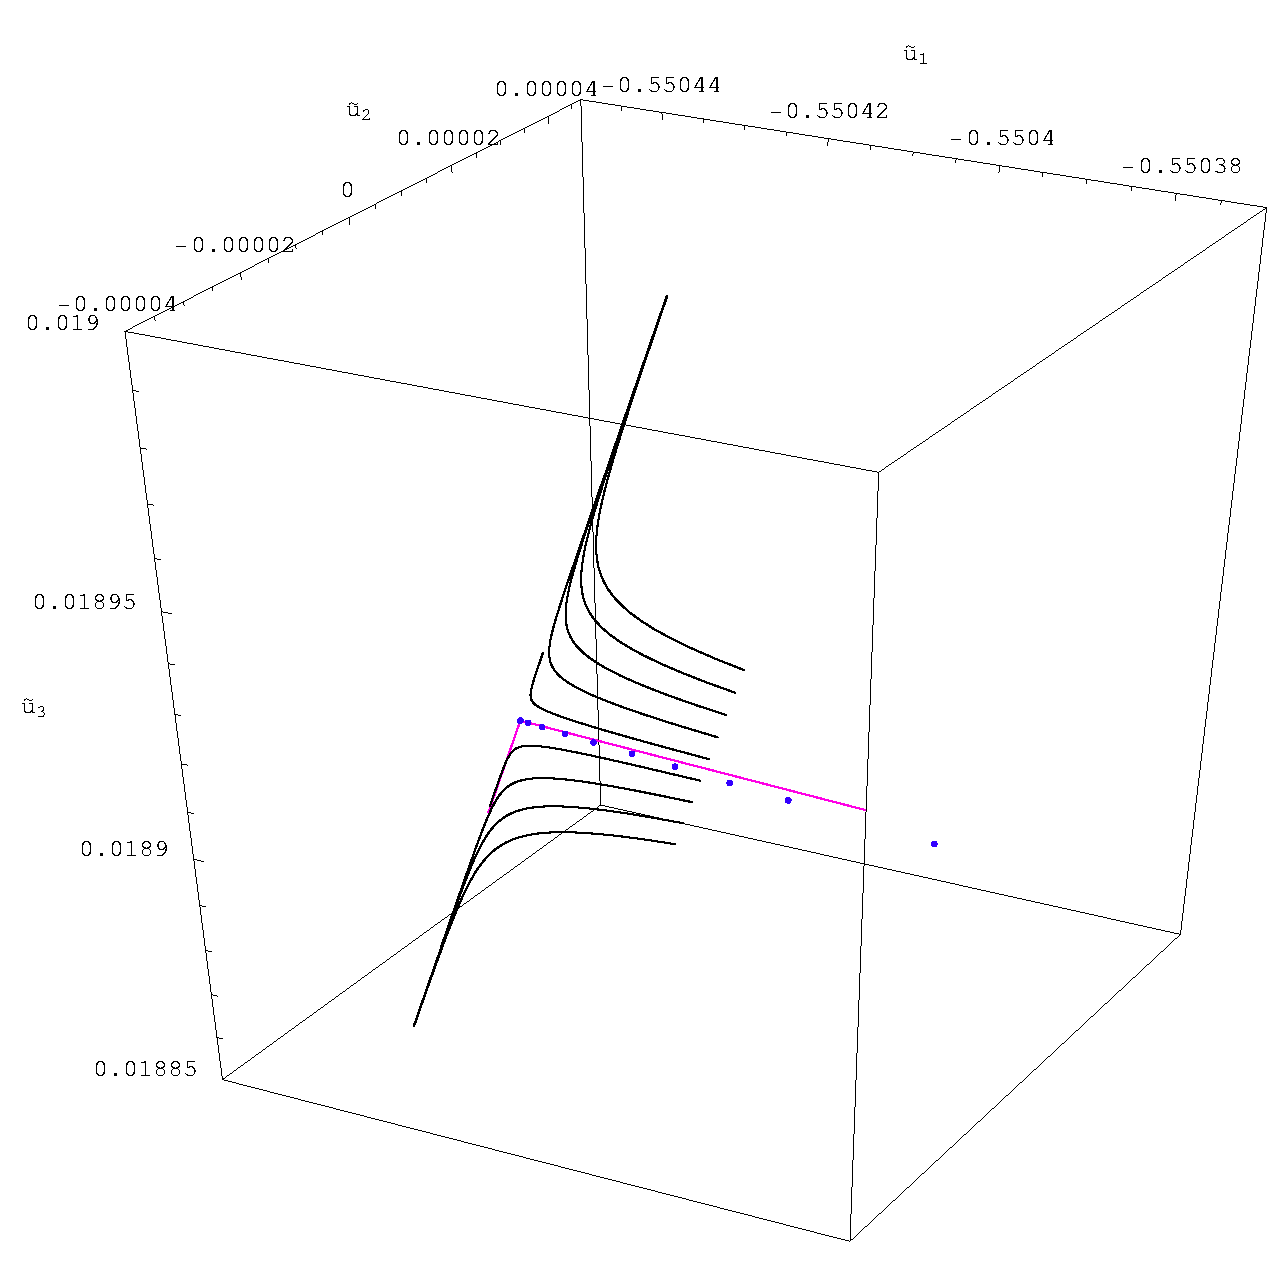
\includegraphics[width=5.0cm]{figs/L22-2w-3w-detail.eps}
% (d) 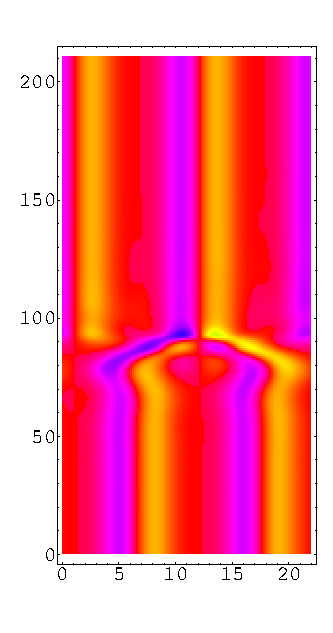
\includegraphics[width=4.0cm]{figs/L22-2w-B.eps}
\caption{
 Trajectories with initial conditions on the unstable subspace of
 the \nameit 2 {\eqva}.  
 (a) The coordinates $\tilde{u}_1$ and $\tilde{u}_2$ are along the directions defining the unstable subspace
 and $\tilde{u}_3$  is along the real part of the eigenvector, 
 corresponding to the eigenvalue $-0.271122+ i\, 0.356307$. The purple points represent the continous family
 of 
\nameit 2 \eqva.
% Green curve belongs to \reffig{f:rpo55}(b) % rpo22-55-4-cm.eps
% rather than to  \reffig{f:rpo55}(a), % rpoEq22-55-4.eps?
(b) blowup of ``homoclinic'' descent of the unstable manifold
back into {\nameit}-2 {\eqv}, shifted by
$L/4 =5.5$.
(c) blowup of ``heteroclinc'' connection from 
{\nameit}2 \eqv\ to {\nameit}3 \eqv\, with shift 
$L(1/3-1/4) = L/12 = 1.83$ (? check)
to the neighborhood of the point near which the
unstable manifold of the 
\nameit 2 \eqv\ splits. The blue points
represent the 
\nameit 3 {\eqv} family.
The descent is along the eigenvector of $\Lyap_4= 0.413$ (checked by ES),
and spliting
occurs along one of the 
$\Lyap_1=\Lyap_2=0.0933$
unstable directions of the \nameit 2 {\eqv} (checked by ES).
d) same as (c), closer to the \nameit 3 {\eqv}. The eigendirections corresponding to $\Lyap_1$
and $\Lyap_4$ are shown in purple. 
}
\label{f:neighborhood2w}
\end{figure}
%%%%%%%%%%%%%%%%%%%%%%%%%%%%%%%%%%%%%%%%%%%%%%%%%%%%%%%%%%%%%%%%%%


\subsection{\Reqva}

Numerical solution of the \reqv\  condition,
transported by travelling wave velocity $c$, 
fixed by the solution for the travelling wave equation:
\[
f_k(u) - i{2\pi\over L} c k u_k = 0
\]

\underline{1-\reqv\  (travelling wave).}
% Ruslan L Davidchack, 	10 Jul 2006 
There is a pair of \reqva\ 
${\nameit}1L$,
${\nameit}1R$
(traveling waves), dual under the
$u(x) \to -u(-x)$ symmetry. They are 
determined numerically by 
adiabatic continuation from a smaller system size
$L~\approx 12$,
where they are stable, to $L=22$
where their velocity is atypically large, $c=7.???$,

Their exponents are:
\\
$\Lyap_i \pm \theta_i =
(
\\
  0.1156222 \pm 0.817289,	\\
  0.033663 \pm 0.418909,	\\
 0.0                    ,	\\
 -0.245729                    ,	\\
 -0.321321 \pm 0.98126,
\cdots
)$

The pair of \reqva\ 
${\nameit}2L$,
${\nameit}2R$
exists for larger system sizes, but does not continue 
adiabatically\rf{saddks} down to $L=22$.


\subsection{\Eqva, $L$ and $c$}

%%%%%%%%%%%%%%%%%%%%%%%%%%%%%%%%%%%%%%%%%%%%%%%%%%%%%%%%%%%%%%%%
\begin{figure}[t]
	% \vspace*{-5pt}
\centering
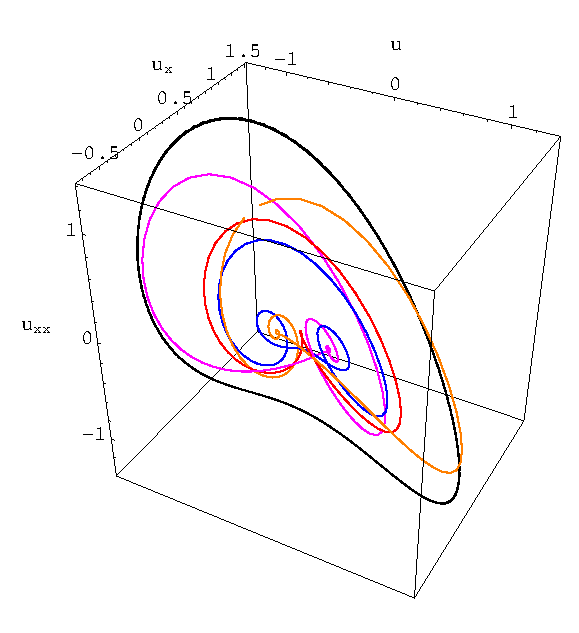
\includegraphics[width=0.6\textwidth]{figs/equilSpatial}
	% \vspace*{-5pt}
\caption{
	{\small
$(u,u_x,u_{xx})$ representation
of $\EQV{1}$ (blue), $\EQV{2}$ (red), $\EQV{3}$ (black) \eqva.
$\tildeL=3.5014$, $N=64$ complex modes truncation.
        } %end \small
        }
\label{f:eqvSpatial}
	% \vspace*{-5pt}
\end{figure}
%%%%%%%%%%%%%%%%%%%%%%%%%%%%%%%%%%%%%%%%%%%%%%%%%%%%%%%%%%%%%%%%%%

\PC{
 add the left/right $\REQV{\pm}{1}$ pair to \reffig{f:eqvSpatial}
    }
The $u=0$  \eqv\ $\EQV{0}$ is a point at the origin
in \reffig{f:eqvSpatial}.
At
each integer value of $\tildeL$ the origin spews out a Hopf cycle. That
might help us prove that we have all equilibria for $L=22$.

Each of these \eqva\ has a different value of the $c$ integration
constant. 

Plot also the two \eqva\ of \eqva\ points, their
real eigenvectors and their complex eigenplanes. All equilibria presumably
wind around these, and as box size $L$ changes, they form continuous
families with smoothly changing $c$. One can check that by
changing $L$ a bit and using the previous equilibrium to find the next
one.

What does the complex eigenplane continuation does for these
equilibria - does it produce nice heteroclinic connections, or is it
wierder? We know there is an analytic formula for a heteroclinic
connection (see \refref{Lan:Thesis}). % Lan's thesis).

THe real motivation for all this is that if we understand \eqva\ as
$L \to \infty$ we might have an entry into $L = \infty$ periodic orbit
theory of KS.


